\documentclass[10pt,a4paper]{article}
\usepackage[utf8]{inputenc}
\usepackage[russian]{babel}
\usepackage[OT1]{fontenc}
\usepackage{amsmath}
\usepackage{amsfonts}
\usepackage{amssymb}
\usepackage{graphicx}
\usepackage{placeins}
\author{Никитина А.В., Замотаева Ю.И.}
\title{Отчет по лабораторным работам по дисциплине ТСС}
\date{2014}
\begin{document}
\maketitle
\pagebreak
\tableofcontents
\pagebreak
\section{Система верстки \TeX и расширения \LaTeX}
\subsection{Цель работы}
Ознакомление с программой для верстки отчетов \TeX.
\subsection{Задача работы}
Научиться создавать титульный лист, разделы, списки и писать несложные формулы в среде верстки отчетов \TeX.
\subsection{Написание математических формул}
\begin{enumerate}
\item
\begin{displaymath}
lim_{n \to \infty}
\sum_{k=1}^n \frac{25}{2*k^3}
= \frac{\pi}{2}
\end{displaymath}
\item 
\begin{displaymath}
x^{3}+\sum_{x=1}^8 \frac{x}{2}
= \sqrt{617}
\end{displaymath}
\item 
\begin{displaymath}
x(t) = A * sin(w*t+f)
\end{displaymath}
\end{enumerate}
Формула интеграла:
\begin{displaymath}
\iint_{\frac{sin(x)}{x}+y^{2} = 1} f(x, y) dx dy 
\end{displaymath}
\subsection{Интерпретация результатов}
Среда верстки отчетов \TeX очень удобна для введения математических формул. Имеется множество команды, которые заметно облегчают ввод дробных выражений, констант, переменных, производных, интегралов, дифференциалов и других формул. Таким образом, можно без особы трудностей вводить формулы различной сложности.
\subsection{Вывод}
В данной лабораторной работе мы познакомились  с системой создания и редактирования текстов \TeX и расширением \LaTeX. Рассмотрели команды этой среды, которые помогают составлять красивые и аккуратные отчеты.
Таким образом, теперь мы без труда может написать отчет, который будет иметь титульный лист, главы, заголовки и различные математические формулы. Нам очень понравилась эта система, потому что она помогает каждому составить отчет быстро и удобно. Система полностью автоматизирована, от нас требуется только освоить основные команды и ознакомиться с дополнительной литературой.

\section{Визуализация сигналов во временной и частотной области}
\subsection{Цель работы}
Познакомиться со средствами генерации сигналов и визуализации их спектров.
\subsection{Постановка задачи}
В командном окне MATLAB и в среде Simulink промоделировать чистый синусоидальный сигнал, так же синусоидальный сигнал с шумом. Получить их спектры.
\subsection{Справочные материалы}
В.С. Гутников Фильтрация измерительных сигналов пп.1-2, 11-12
\subsection{Ход работы}
В среде MATLAB вначале моделируем чистый синусоидальный сигнал по формуле:
\begin{displaymath}
A(t) = A_0sin(2\pi ft + f_0)
\end{displaymath}
Затем моделируем зашумленный сигнал по формуле:
\begin{displaymath}
A(t) = A_0sin(2\pi ft + f_0) + A_1 rand()
\end{displaymath}
Для выделения частот регулярных составляющих используем преобразование Фурье, которое реализовано встроенной в MATLAB функцией.
\subsubsection{Код MATLAB для исходного сигнала}
x=0:0.01:4*pi;\newline
f0 = 20;\newline
\%исходный сигнал\newline
y = sin(2*pi*f0*x);\newline
figure(1)\newline
plot(x(1:200),y(1:200))\newline
grid\newline
\%спектр исходного сигнала\newline
figure(2)\newline
spectrum = fft(y,512);\newline
normspectrum = spectrum.*conj(spectrum)/512;\newline
f=100*(0:255)/512;\newline
plot(f, normspectrum(1:256))\newline
axis([0 max(F) 0 10])\newline
grid\newline
\subsubsection{Результаты работы программы}
В результате выполнения программы получились графики временной и частотной характеристик исходного синусоидальных сигнала.
\begin{itemize}
\item Исходный сигнал
\begin{figure}[h]
\centering
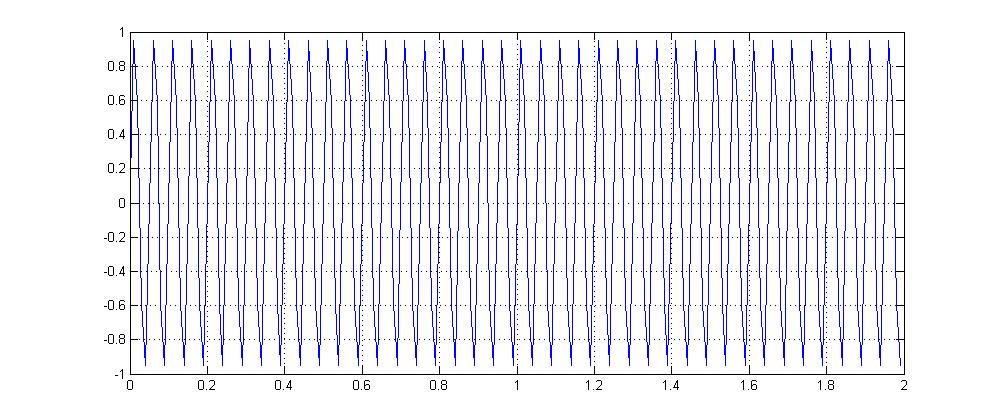
\includegraphics[width=12cm]{1.png} 
\end{figure}
\item Спектр исходного сигнала
\begin{figure}[h]
\centering
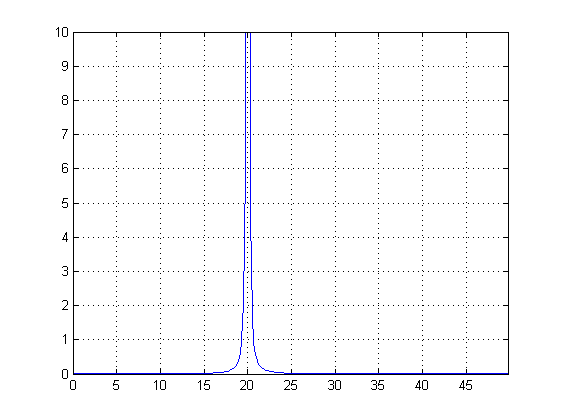
\includegraphics[width=12cm]{2.png} 
\end{figure}
\end{itemize}
\FloatBarrier
\subsubsection{Код MATLAB для зашумленного сигнала}
\%зашумленный сигнал\newline
ynoize = y+ 0.5*rand(size(x));\newline
figure(3)\newline
plot(x(1:200),ynoize(1:200));\newline
grid\newline
\%спектр зашумленного сигнала\newline
spectrum = fft(ynoize,512);\newline
noizespectrum = spectrum.*conj(spectrum)/512;\newline
figure(4)\newline
plot(f, noizespectrum())\newline
axis([0 max(f) 0 10])\newline
grid\newline
\subsubsection{Результаты работы программы}
В результате выполнения программы получились графики временной и частотной характеристик зашумленного синусоидальных сигнала.
\begin{itemize}
\item Зашумленный сигнал
\begin{figure}[h]
\centering
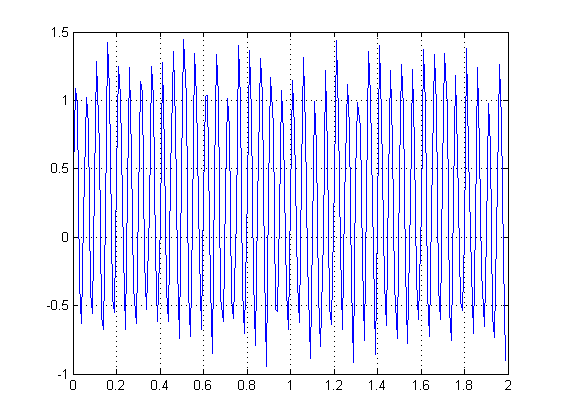
\includegraphics[width=12cm]{3.png} 
\end{figure}
\item Спектр зашумленного сигнала
\begin{figure}[h]
\centering
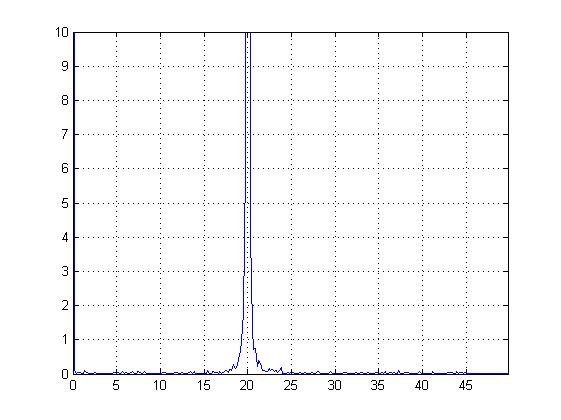
\includegraphics[width=12cm]{4.png} 
\end{figure}
\end{itemize}
\FloatBarrier
\subsection{Вывод}
В данной работе мы построили исходный синусоидальный сигнал, после чего получили его спектр. Спектр представляет из себя резко возрастающий график. Далее построили зашумленный сигнал и его спектр. По рисункам видно, что спектр зашумленного сигнала очень напонимает спектр исходного сигнала, но является более неровным.
Стоит пояснить возможные расхождения между теоретически ожидаемым и полученным спектром сигнала вследствие дискретности представления сигналов, а также их конечности во времени:
Любой сигнал с неограниченным спектром может быть представлен с некоторыми потерями как сигнал с ограниченным спектром.
В силу дискретности представления сигналов мы теряем некоторое количество информации, таким образом, получаем искаженный спектр.
Спектр дискретизированного сигнала получаем в результате сверки непрерывного сигнала с решеткой дельта-импульса.
\begin{displaymath}
S(k*f)=S(f)*\delta(k*f_{n})
\end{displaymath}
А так как мы строим конечный косинус путем умножения на прямоугольное окно, то получаем свертку sin(x)/x, т. е. спектр в виде нескольких(т.к.сигнал дискретизирован) sinc(x).

\section{Спектры простых сигналов}
\subsection{Цель работы}
Получить представление о тестовых сигналах во временной и частотной областях. Реализовать операцию свертки сигналов.
\subsection{Постановка задачи}
В командном окне MATLAB и в среде Simulink промоделировать следующие тестовые сигналы:
\begin{itemize}
\item Полигармонический сигнал 
	\begin{equation}
	y(t) = \sum_{n=0}^{{N}-1}cos{(nt)}
	\end{equation}
\item Прямоугольный импульсный сигнал
	\begin{equation}
	y(t) = \prod(t, T_i)
	\end{equation}
\item Tреугольный импульсный сигнал
	\begin{equation}
	y(t) = \vartriangle(t, T_i)
	\end{equation}
\end{itemize}
и получить их спектры.
\subsection{Справочные материалы}
В.С. Гутников. Фильтрация измерительных сигналов пп.3-6, 13-14
\subsection{Полигормонический сигнал}
\subsubsection{Код Matlab}
x = 0:0.01:4*pi;\newline
f=100*(0:255)/512; \newline
figure\newline
y1 = sin(2*pi*x)+sin(2*pi*3*x);\newline
plot(x(1:200),y1(1:200))\newline
grid\newline
figure\newline
s1 = fft(y1,512);\newline
ss1 = s1.*conj(s1)/512;\newline
plot(f,ss1(1:256))\newline
grid \newline
figure\newline
y2 = sin(2*pi*x)+cos(2*pi*x);  \newline
plot(x(1:200),y2(1:200))  \newline 
grid \newline
figure\newline
s2 = fft(y2,512);\newline
ss2 = s2.*conj(s2)/512;\newline
plot(f,ss2(1:256))\newline
grid \newline
\begin{itemize}
\item полигармонический сигнал sin(x)+sin(3x)
\begin{figure}[h]
\centering
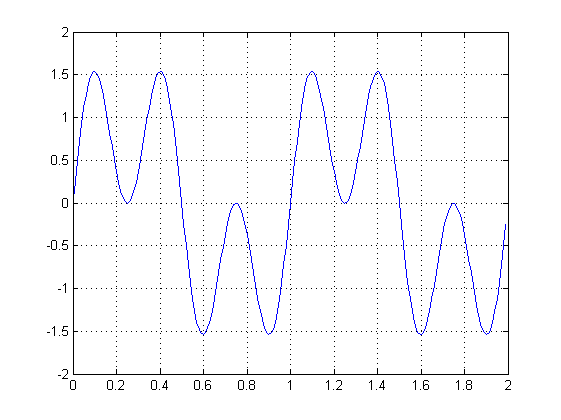
\includegraphics[width=12cm]{5_1.png} 
\end{figure}
\item спектр данного полигармонического сигнала
\begin{figure}[h]
\centering
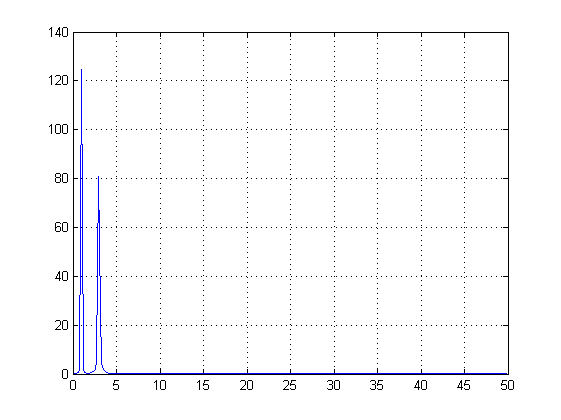
\includegraphics[width=12cm]{5_2.png} 
\end{figure}
\item полигармонический сигнал sin(x)+cos(x)
\begin{figure}[h]
\centering
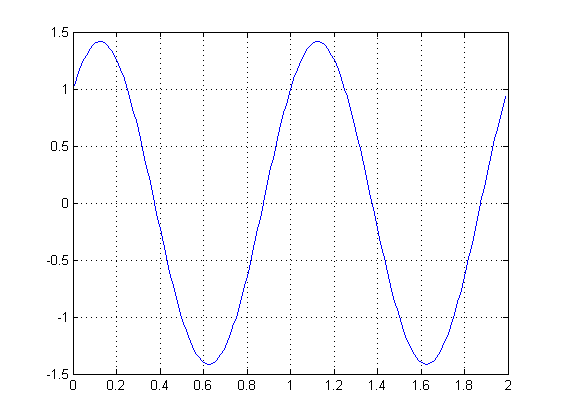
\includegraphics[width=12cm]{12.png} 
\end{figure}
\item спектр данного полигармонического сигнала
\begin{figure}[h]
\centering
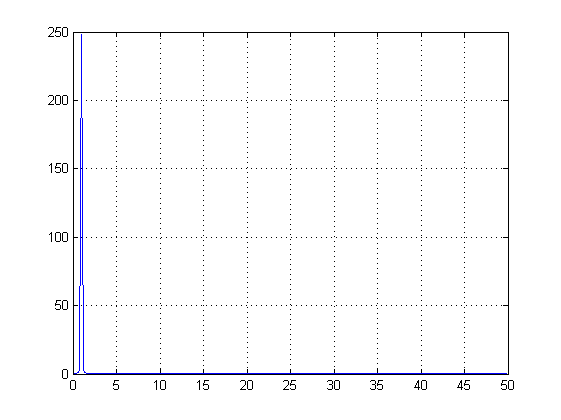
\includegraphics[width=12cm]{11.png} 
\end{figure}
\end{itemize}
\FloatBarrier
\subsubsection{Модуляция в среде Simulink}
\begin{itemize}
\item модель
\begin{figure}[h]
\centering
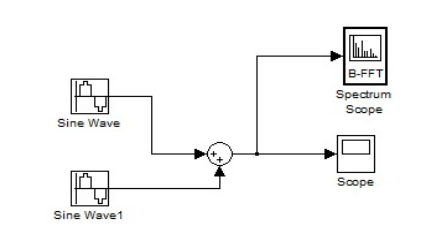
\includegraphics[width=12cm]{sim5_1.png} 
\end{figure}
\item сигнал
\begin{figure}[h]
\centering
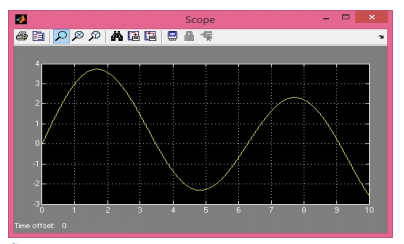
\includegraphics[width=12cm]{sim5_2.png} 
\end{figure}
\item спектр
\begin{figure}[h]
\centering
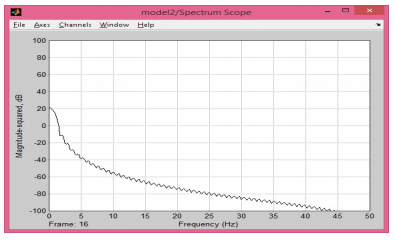
\includegraphics[width=12cm]{sim5_3.png} 
\end{figure}
\end{itemize}
\FloatBarrier
\subsection{Прямоугольный импульсный сигнал}
\subsubsection{Код Matlab}
t=-0.04:1/1000:0.04;\newline
y4=-5*rectpuls(t,0.04);\newline
plot(t,y4);\newline
figure;\newline
spectrum = abs(fft(y4,1024))/1024;\newline
plot(spectrum);\newline
\begin{itemize}
\item Прямоугольный импульсный сигнал
\begin{figure}[h]
\centering
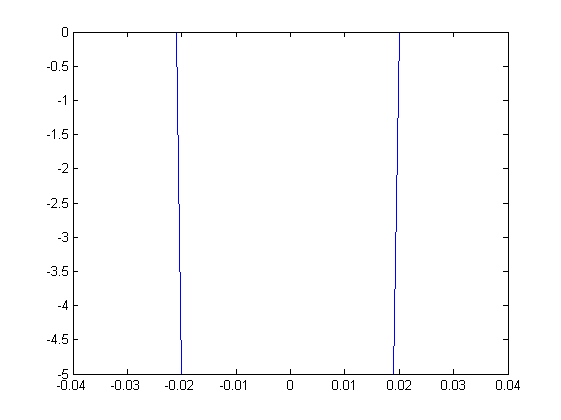
\includegraphics[width=12cm]{5_3.png} 
\end{figure}
\item Спектр прямоугольного сигнала
\begin{figure}[h]
\centering
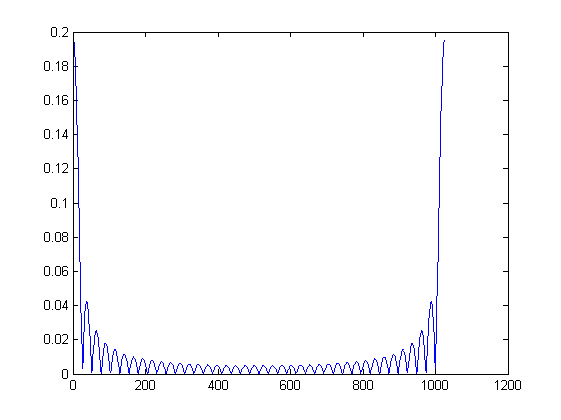
\includegraphics[width=12cm]{5_4.png} 
\end{figure}
\end{itemize}
\FloatBarrier
\subsubsection{Модуляция в среде Simulink}
\begin{itemize}
\item модель
\begin{figure}[h]
\centering
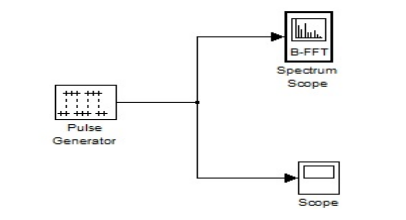
\includegraphics[width=12cm]{sim5_4.png} 
\end{figure}
\item сигнал
\begin{figure}[h]
\centering
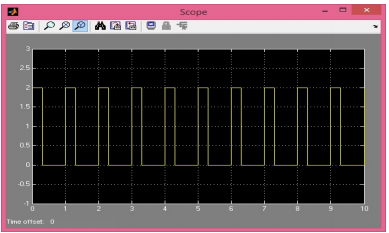
\includegraphics[width=12cm]{sim5_5.png} 
\end{figure}
\item спектр
\begin{figure}[h]
\centering
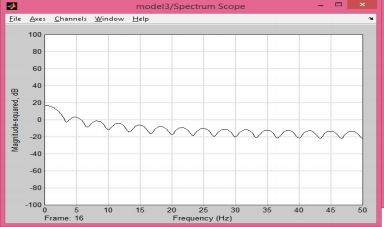
\includegraphics[width=12cm]{sim5_6.png} 
\end{figure}
\end{itemize}
\FloatBarrier
\subsection{Трегольный импульсный сигнал}
\subsubsection{Код Matlab}
t=-0.04:1/1000:0.04;\newline
y4=-5*rectpuls(t,0.02);\newline
y5=-10*rectpuls(t,0.03);\newline
y6= conv(y4,y5);\newline
plot(y6);\newline
figure;\newline
spectrum = abs(fft(y6,1024))/1024;\newline
plot(spectrum);\newline
\begin{itemize}
\item Треугольный импульсный сигнал
\begin{figure}[h]
\centering
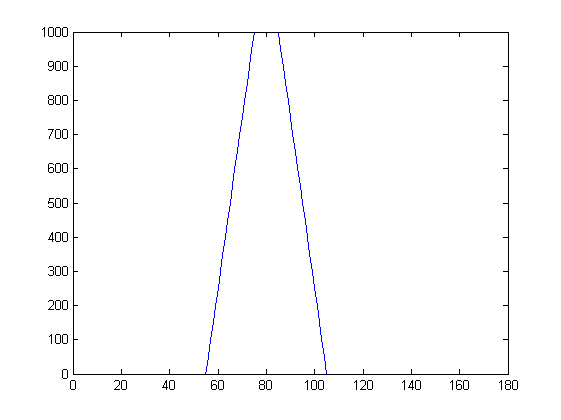
\includegraphics[width=12cm]{5.png} 
\end{figure}
\item Спектр треугольного сигнала
\begin{figure}[h]
\centering
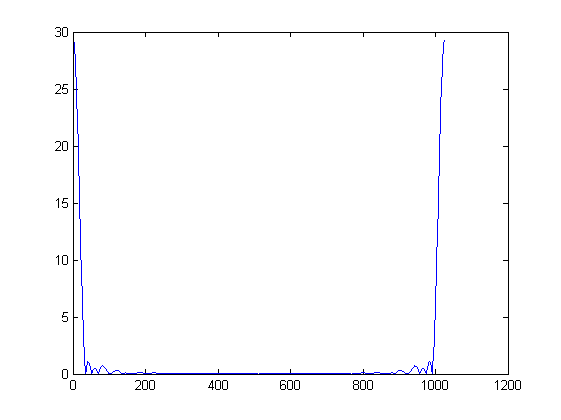
\includegraphics[width=12cm]{6.png} 
\end{figure}
\end{itemize}
\FloatBarrier
\subsubsection{Модуляция в среде Simulink}
\begin{itemize}
\item модель
\begin{figure}[h]
\centering
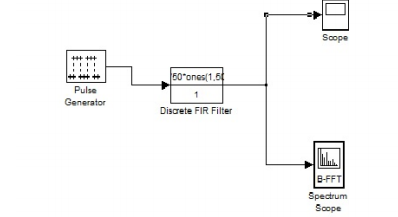
\includegraphics[width=12cm]{sim5_7.png} 
\end{figure}
\item сигнал
\begin{figure}[h]
\centering
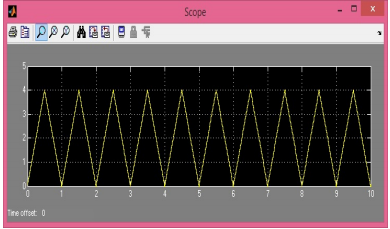
\includegraphics[width=12cm]{sim5_8.png} 
\end{figure}
\item спектр
\begin{figure}[h]
\centering
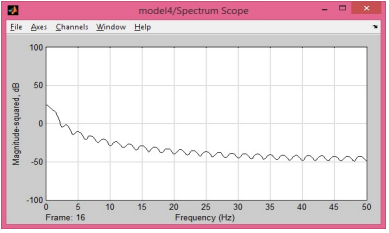
\includegraphics[width=12cm]{sim5_9.png} 
\end{figure}
\end{itemize}
\FloatBarrier
\subsection{Вывод}
В лабораторной работе было проведено моделирование в среде MatLAB и Simulink полигармонического, прямоугольного и треугольного сигналаов. После чего получены их спектры. Для получения сигналов использовались математические формулы данных функций. Треугольный сигнал был получен путем применения операции свертки для двух прямоугольных сигналов. Данная операция осуществляется с помощью специальной функции Matlab. В Simulink для получения генератора треугольного сигнала используется генератор прямоугольных импульсов каскадно с фильтром с прямоугольным окном.\newline
Обоснованием получения треугольного сигнала из свертки двух прямоугольных служит тот факт, что интеграл от произведения двух констант есть линейная функция. График такого преобразования будет представлять две линеные функции, одна из которых имеет положительный коэффициент наклона, а другая отрицательный.
\subsection{Формулы}
Ниже приведены формулы для вычисления спектров исходных импульсов. Так как треугольный импульс можно представить в виде свертки двух прямоугольных, спектр треугольного испульса выражается через квадрат спектра прямоугольного импульса. 
\begin{displaymath}
S(t)=\sum \limits_{k=0}^{K}(a_{k}*cos(2*pi*k*f*t)+b_{k}*sin(2*pi*k*f*t))\newline
\end{displaymath}
\begin{figure}[h]
\centering
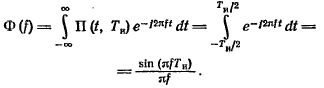
\includegraphics[width=10cm]{8.png} 
\caption{Спектр прямоугольного импульса} 
\end{figure}
\FloatBarrier
\begin{figure}[h]
\centering
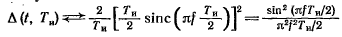
\includegraphics[width=10cm]{9.png} 
\caption{Спектр треугольного импульса} 
\end{figure}
\section{Линейная фильтрация}
\subsection{Цель работы}
Изучить воздействия ФНЧ на тестовый сигнал с шумом. Сгенерировать гармонический сигнал с шумом и синтезировать ФНЧ. Получить сигнал во временной и частотной областях до и после фильтрации.
\subsection{Ход работы}
Линейный фильтр — динамическая система, применяющая некий линейный оператор ко входному сигналу для выделения или подавления определённых частот сигнала и других функций по обработке входного сигнала. 
Фильтр Баттерворта — один из типов электронных фильтров. Фильтры этого класса отличаются от других методом проектирования. Фильтр Баттерворта проектируется так, чтобы его амплитудно-частотная характеристика была максимально гладкой на частотах полосы пропускания. 

 В командном окне Matlab сгенерируем гармонический сигнал без шума и с шумом, а также спектры сигнала с шумом и без шума. В результате код Matlabа будет выглядеть так:
\begin{verbatim}
x = 0:0.01:4*pi;
f=100*(0:255)/512;
figure
noise=rand(size(x));
y = sin(2*pi*x);
y_noisy = y+0.3*noise;

%Построение сигнала без шума:
plot(x(1:200),y(1:200))
grid

%Построение сигнала с шумом:
plot(x(1:200),y_noisy(1:200))
grid

%синтез ФНЧ Баттерворта
[B,A] = butter(16,0.99);
B=B./sum(B);
A=A./sum(A);
%обработка сигнала ФНЧ
figure
y_filtered = conv(y_noisy,[B,A]);

%Построение сигнала после прохождения через фильтр:
plot(x(1:200),y_filtered(1:200))
grid
figure
%Построение спектра сигнала с шумом
noisy_spectrum = fft(y_noisy,512);
norm_noisy_spectrum = noisy_spectrum.*conj(noisy_spectrum)/512;

%Построение нормирова спектра сигнала с шумом:
plot(f,norm_noisy_spectrum(1:256))
axis([0 max(f) 0 2])
grid
figure

%Спектр отфильтрованного сигнала
spectrum = fft(y_filtered,512);
norm_filtered_spectrum=spectrum.*conj(spectrum)/512;
%Построение нормированого отфильтрованного спектра:
plot(f,norm_filtered_spectrum(1:256))
axis([0 max(f) 0 2])
grid
\end{verbatim}
Результаты работы программы на рисунке.
\begin{figure}[H]
\begin{minipage}[h]{0.6\linewidth}
\center{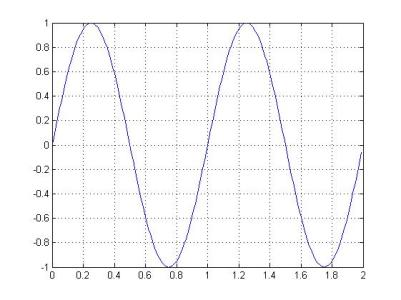
\includegraphics[width=1\linewidth]{im1}} a) \\
\end{minipage}
\vfill
\begin{minipage}[h]{0.6\linewidth}
\center{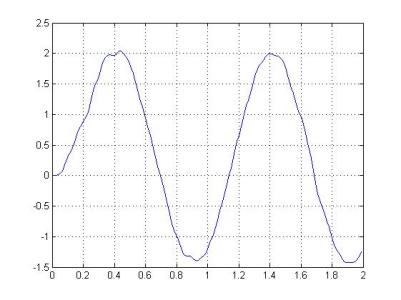
\includegraphics[width=1\linewidth]{im2}} \\б)
\end{minipage}
\hfill
\begin{minipage}[h]{0.6\linewidth}
\center{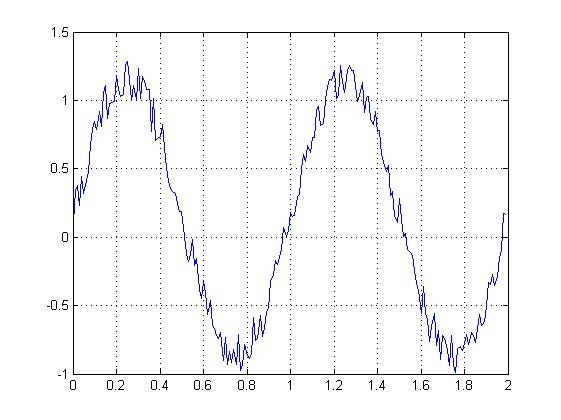
\includegraphics[width=1\linewidth]{im56}} в) \\
\end{minipage}

\vfill
\begin{minipage}[h]{0.6\linewidth}
\center{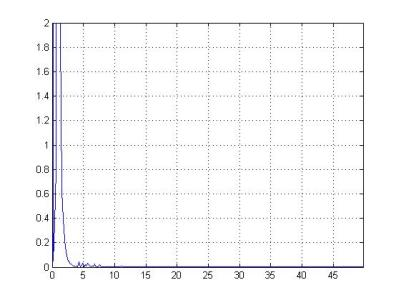
\includegraphics[width=1\linewidth]{im4}} г) \\
\end{minipage}
\hfill
\begin{minipage}[h]{0.6\linewidth}
\center{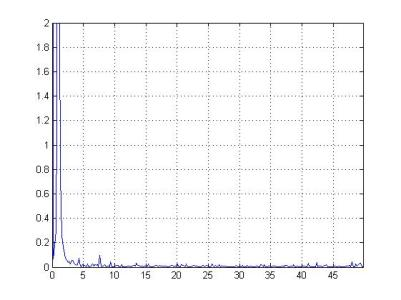
\includegraphics[width=1\linewidth]{im3}} д) \\
\end{minipage}
\caption{Линейная фильтрация в Matlab: a) Сигнал без шума, б)
Сигнал после фильтрации, в)Сигнал с шумом, г)Спектр сигнала после фильтрации, д)Спектр сигнала с шумом.}
\label{ris:experimentalcorrelationsignals}
\end{figure}
\FloatBarrier
\subsection{Моделирование в Simulink}
Для создания модели в Simulink используем блок Discrete FIR Filter раздела Discrete главной библиотеки и блок Digital Filter design из Signal Processing Blockset/Filtering/Filter Designs. Результаты моделирование в Simulink на рисунке.
\begin{figure}[H]
\begin{minipage}[h]{0.6\linewidth}
\center{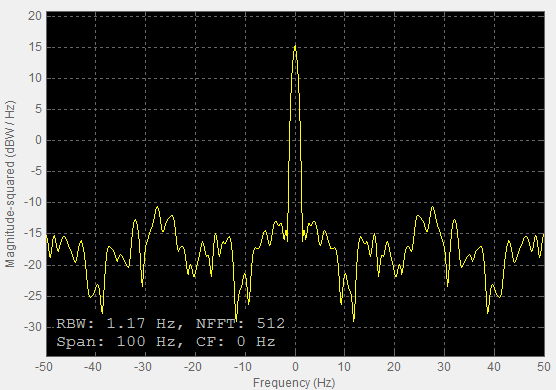
\includegraphics[width=1\linewidth]{im7}} a) \\
\end{minipage}
\hfill
\begin{minipage}[h]{0.6\linewidth}
\center{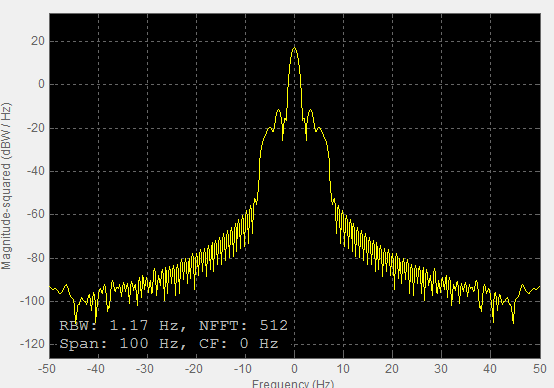
\includegraphics[width=1\linewidth]{im6}} \\б)
\end{minipage}
\vfill
\begin{minipage}[h]{0.6\linewidth}
\center{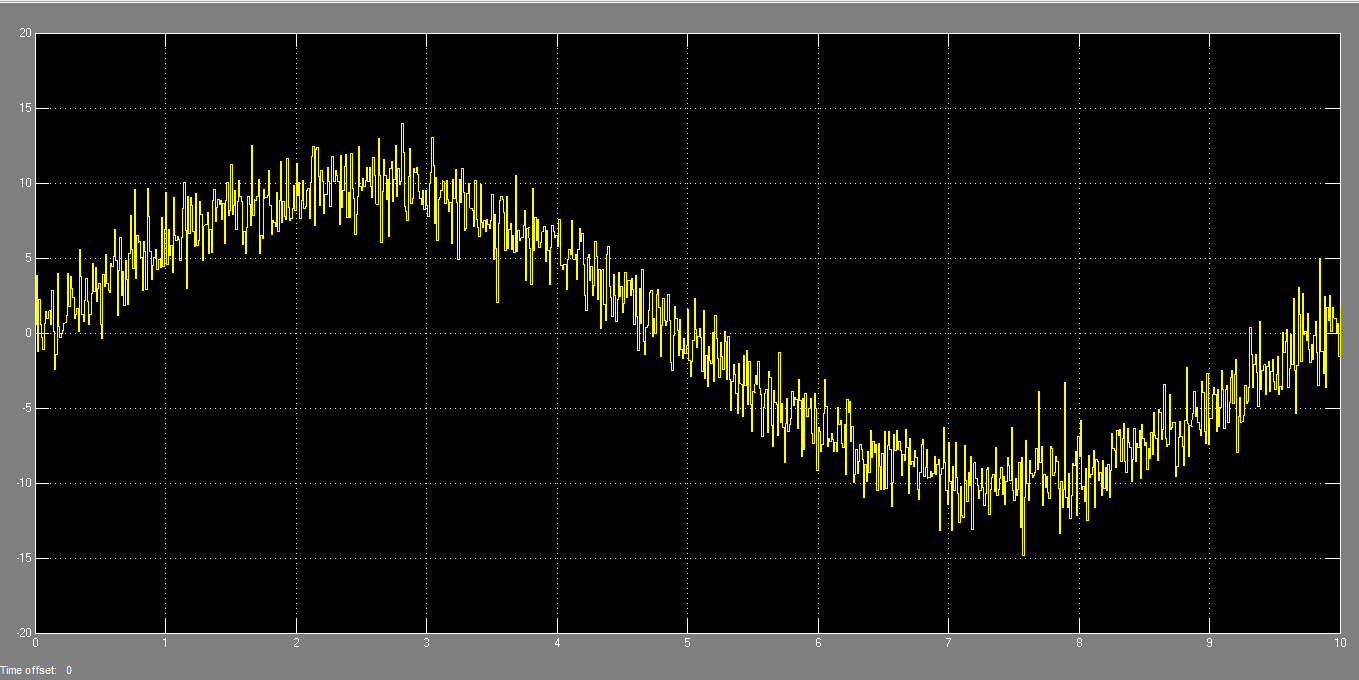
\includegraphics[width=1\linewidth]{im8}} в) \\
\end{minipage}
\hfill
\begin{minipage}[h]{0.6\linewidth}
\center{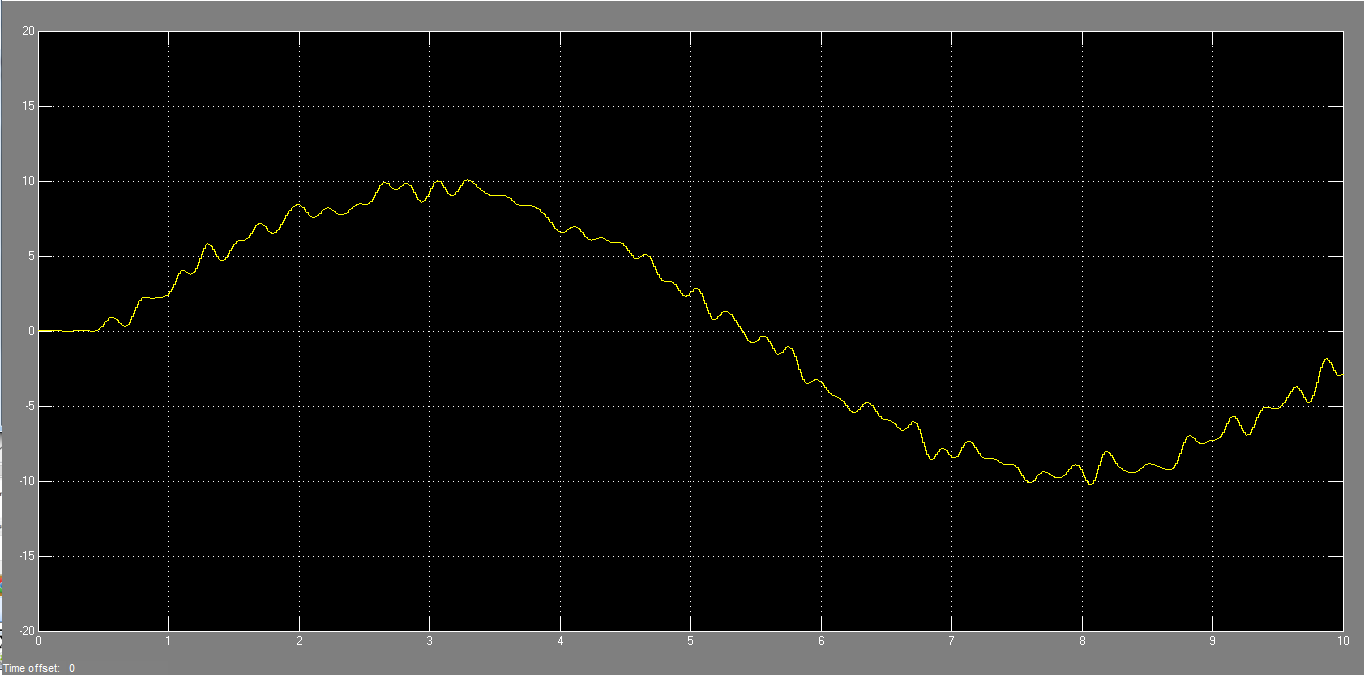
\includegraphics[width=1\linewidth]{im9}} г) \\
\end{minipage}
\hfill
\begin{minipage}[h]{0.6\linewidth}
\center{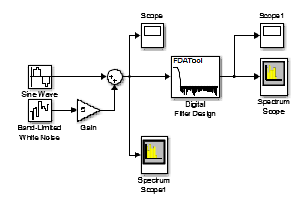
\includegraphics[width=1\linewidth]{im5}} д) \\
\end{minipage}
\caption{Линейная фильтрация в Simulink: a) Спектр до фильтрации, б)
Спектр после фильтрации, в)Сигнал до фильтрации, г)Сигнал после фильтрации, д) Схема модели.}
\label{ris:experimentalcorrelationsignals}
\end{figure}
\FloatBarrier
\subsection{Вывод}
Фильтр нижних частот — один из видов аналоговых или электронных фильтров, эффективно пропускающий частотный спектр сигнала ниже некоторой частоты (частоты среза), и уменьшающий (подавляющий) частоты сигнала выше этой частоты. Степень подавления каждой частоты зависит от вида фильтра. В лабораторной работе мы произвели неполное удаление шума линейным фильтром. Для его полного удаления нам необходим идеальный фильтр (с прямоугольным окном). Линейная фильтрация не устраняет полностью шум, т.к. для полного удаления необходим идеальный фильтр с прямоугольным окном, которого на практике не существует. Так же, т. к. линейный фильтр подавляет все сигналы, находящиеся в его полосе задержания и не изменяет сигналы из полосы пропускания, то он не может удалить шум, который попал в его полосу 
пропускания. Соответственно удалить весь шум он не в силах. 
\section{Аналоговая модуляция}
\subsection{Цель работы}
Изучить процесс амплитудной модуляции/демодуляции сигнала.
\subsection{Алгоритм работы}
\begin{itemize}
\item Сгенерировать однотональный сигнал низкой частоты.
\item Выполнить амплитудную модуляцию (АМ) сигнала по закону 
\begin{displaymath}
u(t)=(1+M*U_{m}*cos(\Omega*t))*cos(\omega_{0}*t+\phi_{0})\newline
\end{displaymath}
  для различных значений глубины модуляции M.
\item Получить спектр модулированного сигнала.
\item Выполнить модуляцию с подавлением несущей: 
\begin{equation}
	u(t) = MU_m cos(\omega t)cos(\omega_0 t+\phi_0).
          \end{equation}
Получить спектр.
\item Выполнить однополосную модуляцию:
\begin{equation}
  u(t) = U_m cos(\omega t)cos(\omega_0 t+\phi_0)+\frac{U_m}{2}\sum_{n=1}^N M_n (cos(\omega_0 + \Omega_n )t + \phi_0 + \Phi_n ),
  \end{equation}
положив n = 1.
\item Выполить синхронное детектирование и получить исходный однополосный сигнал.
\item Рассчитать КПД модуляции:
\begin{equation}
					\eta_A M = \frac{U_m ^2 M^2 /4}{P_U} = \frac{M^2}{M^2 + 2}.
				\end{equation}
\end{itemize}
\subsection{Теоретические сведения}
Перенос спектра сигналов из низкочастотной области в выделенную для их передачи область высоких частот выполняется операцией модуляции.
АМ соответствует переносу информации s(t)=>U(t) при постоянных значениях параметров несущей частоты. АМ – сигнал представляет собой произведение информационной огибающей U(t)  и гармонического колебания ее заполнения с более высокими частотами.
Форма записи амплитудно-модулированного сигнала:
\begin{displaymath}
u(t)=(1+M*U_{m}*cos(\Omega*t))*cos(\omega_{0}*t+\phi_{0})\newline
\end{displaymath}
, где U – постоянная амплитуда несущего колебания при отсутствии входного (модулирующего) сигнала s(t), M  – коэффициент амплитудной модуляции. Значение  M характеризует глубину амплитудной модуляции. В зависимости от значения  M различают нормальную модуляцию ( M<1 ), глубокую модуляцию ( M=1 ) и перемодуляцию ( M>1 ).
КПД амплитудной модуляции равен 
\begin{displaymath}
\eta_{A}*M=\frac{M^{2}}{M^{2}+2}
\end{displaymath}
Как видно, основная доля мощности АМ – сигнала приходится на несущую частоту. При балансной модуляции (с подавлением несущей) производится перемножение двух сигналов – модулирующего и несущего, при котором происходит подавление несущего колебания, соответственно, КПД модуляции становится равным 100%. Так, для однотонального сигнала (без учета начальных фаз колебаний) при 
\begin{displaymath}
u(t)=M*cos(\Omega*t))
\end{displaymath}  имеем
\begin{displaymath}
u(t)=M*U_{m}*cos(\Omega*t)*cos(\omega_{0}*t)=U_{m}*\frac{M}{2}*(cos((\omega_{0}+\Omega)*t)+cos((\omega_{0}-\Omega)*t)))
\end{displaymath}
 , т.е. два одинаковых по амплитуде гармонических сигнала с верхней и нижней боковыми частотами. По существу, однотональный модулирующий сигнал переносится на две высокие частоты.
\subsection{Код MATLAB для п.1-3}
f0=3; частота сигнала \newline
fd=150; частота дискретизации\newline
fc=30; частота несущего колебания\newline
x=0:0.01:4*pi;\newline
y=0.5*sin(2*pi*f0*x);\newline
plot(x(1:200),y(1:200))\newline
grid;\newline
figure\newline
M1=0.3; \newline
M2=1;\newline
M3=1.3;\newline
t=0:0.001:10;\newline
Um=0.5;\newline
f=100*(0:255)/512;\newline
u1=(1+Um*M1*cos(f0*t)).*cos(fc*t); модулированный сигнал\newline
plot(t,u1)\newline
figure\newline
s1=fft(u1,512); спектр модулированного сигнала\newline
ss1=s1.*conj(s1)/512;\newline
plot(f,ss1(1:256));\newline
figure\newline
u2=Um*(1+M2*cos(f0*t)).*cos(fc*t);\newline
plot(t,u2)\newline
figure\newline
s2=fft(u2,512);\newline
ss2=s2.*conj(s2)/512;\newline
plot(f,ss2(1:256));\newline
figure\newline
u3=Um*(1+M3*cos(f0*t)).*cos(fc*t);\newline
plot(t,u3)\newline
figure\newline
s3=fft(u3,512);\newline
ss3=s3.*conj(s3)/512;\newline
plot(f,ss3(1:256));\newline
\begin{figure}[h]
\centering
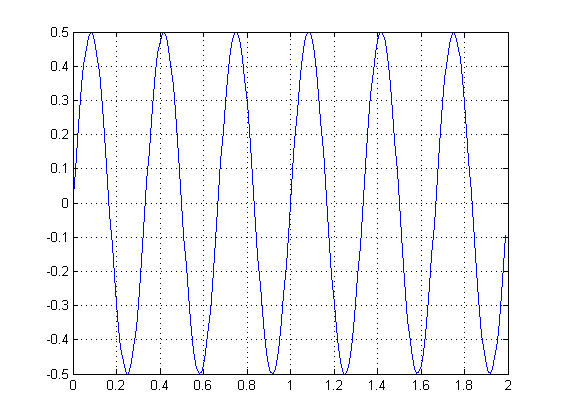
\includegraphics[width=12cm]{am1_1.png} 
Исходный низкочастотный сигнал
\end{figure}
\FloatBarrier
\begin{figure}[H]
\begin{minipage}[h]{0.6\linewidth}
\center{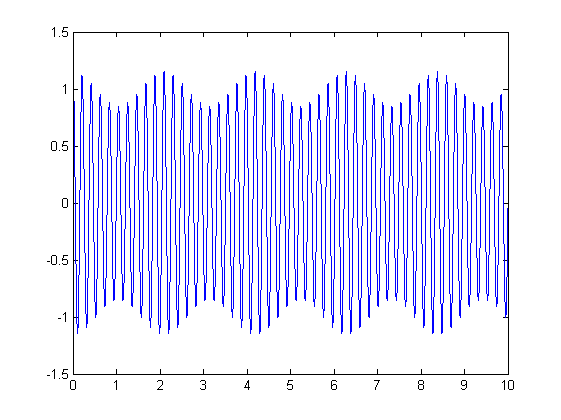
\includegraphics[width=1\linewidth]{am1_2}} а)\\
\end{minipage}
\hfill
\begin{minipage}[h]{0.6\linewidth}
\center{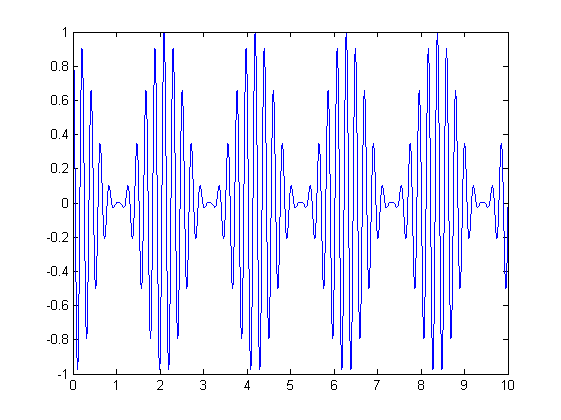
\includegraphics[width=1\linewidth]{am1_4}} б) \\
\end{minipage}
\hfill
\begin{minipage}[h]{0.6\linewidth}
\center{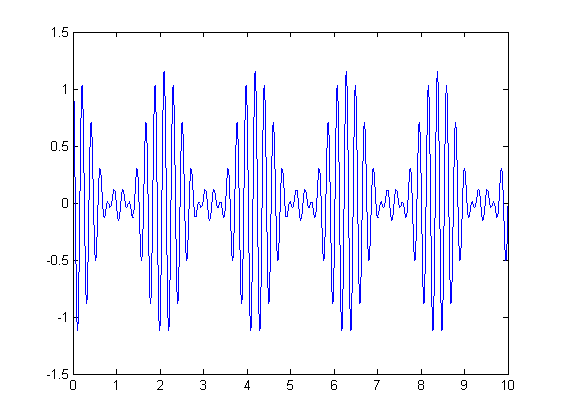
\includegraphics[width=1\linewidth]{am1_6}} в) \\
\end{minipage}
\hfill
\begin{minipage}[h]{0.6\linewidth}
\center{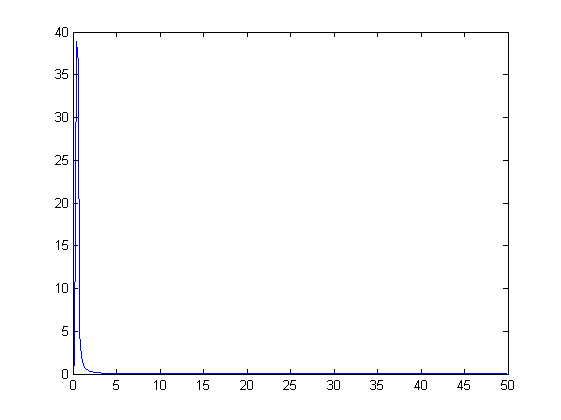
\includegraphics[width=1\linewidth]{am1_5}} г) \\
\end{minipage}
\begin{minipage}[h]{0.6\linewidth}
\center{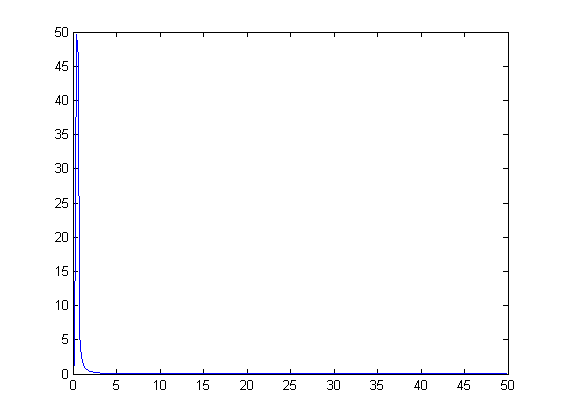
\includegraphics[width=1\linewidth]{am1_7}} д) \\
\end{minipage}
\begin{minipage}[h]{0.6\linewidth}
\center{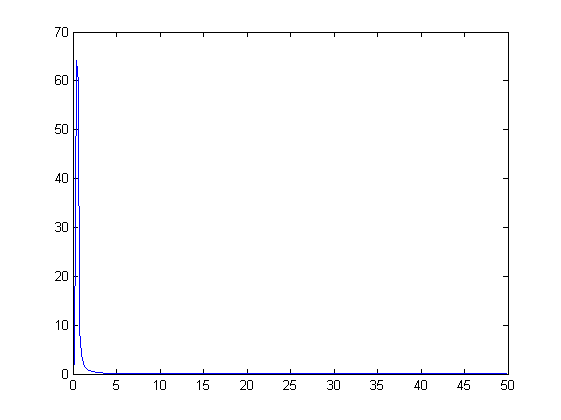
\includegraphics[width=1\linewidth]{am1_3}} е) \\
\end{minipage}
\caption{Линейная фильтрация в Simulink: а)
АМ при степени глубины=0.3, б)АМ при степени глубины=1, в)АМ при степени глубины=1.3, г) Спектр модулированного сигнала при степени глубины=0.3, д) Спектр модулированного сигнала при степени глубины=1, е) Спектр модулированного сигнала при степени глубины=1.3.}
\label{ris:experimentalcorrelationsignals}
\end{figure}
\FloatBarrier
\subsection{Код MATLAB для п.4}
 plot(x(1:200),y(1:200)) исходный сигнал\newline
grid;\newline
figure\newline
u4=Um*M1*cos(f0*t).*cos(fc*t); модуляция с подавлением несущей\newline
plot(t,u4) \newline
figure\newline
s4=fft(u4,512);\newline
ss4=s4.*conj(s4)/512;\newline
plot(f,ss4(1:256));
figure\newline
plot(t,YY);\newline
\begin{figure}[H]
\begin{minipage}[h]{0.6\linewidth}
\center{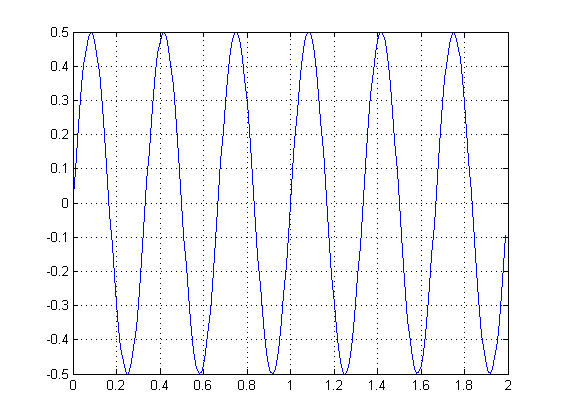
\includegraphics[width=1\linewidth]{am1_1}} а)\\
\end{minipage}
\hfill
\begin{minipage}[h]{0.6\linewidth}
\center{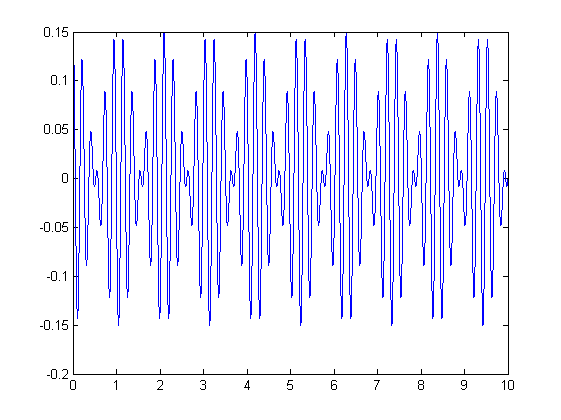
\includegraphics[width=1\linewidth]{am2_2}} б) \\
\end{minipage}
\hfill
\begin{minipage}[h]{0.6\linewidth}
\center{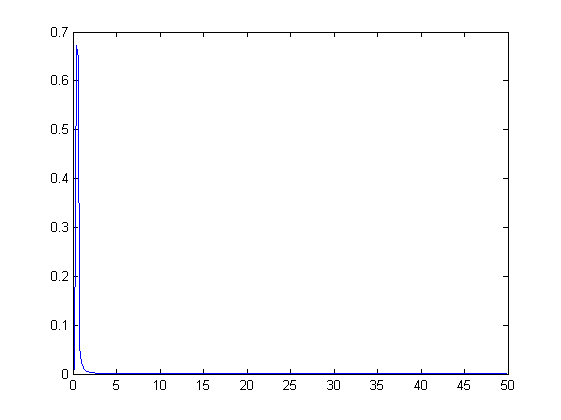
\includegraphics[width=1\linewidth]{am2_3}} в) \\
\end{minipage}
\hfill
\caption{Линейная фильтрация в Simulink: а)
Исходный низкочастотный сигнал, б)Модулированный сигнал с подавлением несущей, в) Спектр модулированного сигнала с подавлением несущей.}
\label{ris:experimentalcorrelationsignals}
\end{figure}
\FloatBarrier
\subsection{Код MATLAB для п.5}
 x=0:0.01:4*pi;\newline
y=sin(2*pi*2*x); \newline
plot(x(1:200),y(1:200),'r')\newline 
t=0:0.001:10;\newline
u2=(1+1*cos(2*t)).*cos(20*t);\newline
s2=fft(u2,512);\newline
yy=u2.*cos(20*t);\newline
plot(t,yy,'r');\newline
ss=fft(yy,512);\newline
sss=ss.*conj(ss)/512;\newline
plot(f,sss(1:256),'r');\newline
\begin{figure}[H]
\begin{minipage}[h]{0.8\linewidth}
\center{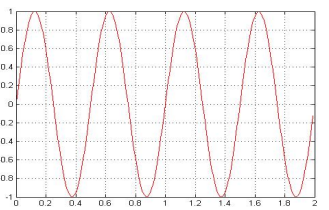
\includegraphics[width=1\linewidth]{am3_3}} а)\\
\end{minipage}
\vfill
\begin{minipage}[h]{0.8\linewidth}
\center{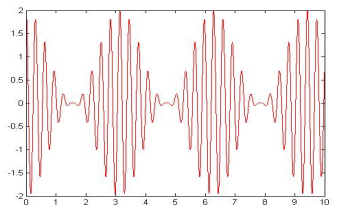
\includegraphics[width=1\linewidth]{am3_1}} б) \\
\end{minipage}
\vfill
\begin{minipage}[h]{0.8\linewidth}
\center{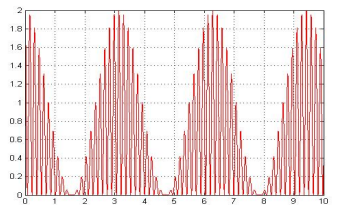
\includegraphics[width=1\linewidth]{am3_2}} б) \\
\end{minipage}
\vfill
\caption{Линейная фильтрация в Simulink: а)
Исходный сигнал, б)Модулированный сигнал, в)Сигнал после выполнения синхронного детектирования.}
\label{ris:experimentalcorrelationsignals}
\end{figure}
\FloatBarrier
\subsection{Код MATLAB для п.6}
Найдем КПД модуляции по формуле
\begin{displaymath}
\eta_{A}*M=\frac{M^{2}}{M^{2}+2}
\end{displaymath}
\begin{center}
M=0.3; КПД=0.14\newline
M=1; КПД=0.3(3)\newline
M=1.3; КПД=0.35\newline
\end{center}
\subsection{Вывод}
Для однотональной модуляции начальная фаза модулирующего колебания для верхней боковой частоты складывается с начальной фазой несущей, для нижней – вычитаются из фазы несущей.
При балансной модуляции производится перемножение двух сигналов – модулирующего и несущего, при котором происходит подавление несущего колебания, соответственно, КПД модуляции становится равным 100%.
\section{Частотная и фазовая модуляция}

\subsection{Цель работы}
Изучение частотной и фазовой модуляции/демодуляции сигнала.

\subsection{Постановка задачи}
	\begin{enumerate}
		\item Сгенерировать однотоальный сигнал низкой частоты.
		\item Выполнить фазовую модуляцию/демодуляцию сигнала по закону
				\begin{equation}
					u(t) = U_m cos(\Omega t + ks(t)),
				\end{equation}
		используюя встроенную функцию MatLab pmmod, pmdemod.
		\item Получить спектр модулированного сигнала.
		\item Выполнить частотню модуляцию/демодуляцию по закону
				\begin{equation}
					u(t) = U_m cos(\omega_0 t + k \int_0^t s(t) dt + \phi_0),
				\end{equation}
		используюя встроенные функции MatLab fmmod, fmdemod.
	\end{enumerate}

\subsection{Справочные материалы}
Н.В. Богач и др. Обработка сигналов в информационных системах, с. 118-125, 127-133.

\subsection{Ход работы}
Фазовая модуляция – процесс изменения мгновенной фазы несущего колебания пропорционально изменению непрерывного информационного сигнала. Фазомодулированный сигнал s(t) имеет следующий вид:
	\begin{equation}
	s(t) = g(t) \sin[2 \pi f_c t + \varphi(t)],
	\end{equation}
где g(t) — огибающая сигнала; $\varphi(t)$ является модулирующим сигналом; $f_c$ — частота несущего сигнала; t — время.
В случае, когда информационный сигнал является дискретным, то говорят о фазовой манипуляции.

По характеристикам фазовая модуляция близка к частотной модуляции. В случае синусоидального модулирующего (информационного) сигнала, результаты частотной и фазовой модуляции совпадают.

Реализация фазовой модуляции/демодуляции с помощью MATLAB:
\begin{verbatim}
% Исходный сигнал
x = 0:0.01:4*pi;
y = sin(2*pi*x);

figure
subplot(4, 1, 1);
plot(x(1:500), y(1:500))
grid
title('Исходный сигнал')
 
% Фазовоя модуляция
Fs = 1000;                      % Частота дискретизации 
Fc = 4;                         % Несущая частота 
phasedev = pi/2;                % Девиация фазы для фазовой модуляции
pm_y = pmmod(x,Fc,Fs,phasedev); % Фазовая модуляция
subplot(4, 1, 2);
plot(x(1:500), pm_y(1:500))
grid
title('Фазовая модуляция')

spectrum = fft(pm_y, 512);      % Спектр фазовой модуляции
norm_spectrum = spectrum.*conj(spectrum)/512;  
f = 100*(0:255)/512;
subplot(4, 1, 3);
plot(f, norm_spectrum(1:256))
grid
title('Спектр фазовой модуляции')
axis([min(f) max(f) 0 max(norm_spectrum)]);

pdm_y = pmdemod(pm_y,Fc,Fs,phasedev); % Демодуляция
subplot(4, 1, 4);
plot(x, pdm_y)
grid
title('Фазовая демодуляция')
\end{verbatim}


В результате выполнения приведенного кода были получены следующие характеристики:

\begin{figure}[h]\centering
	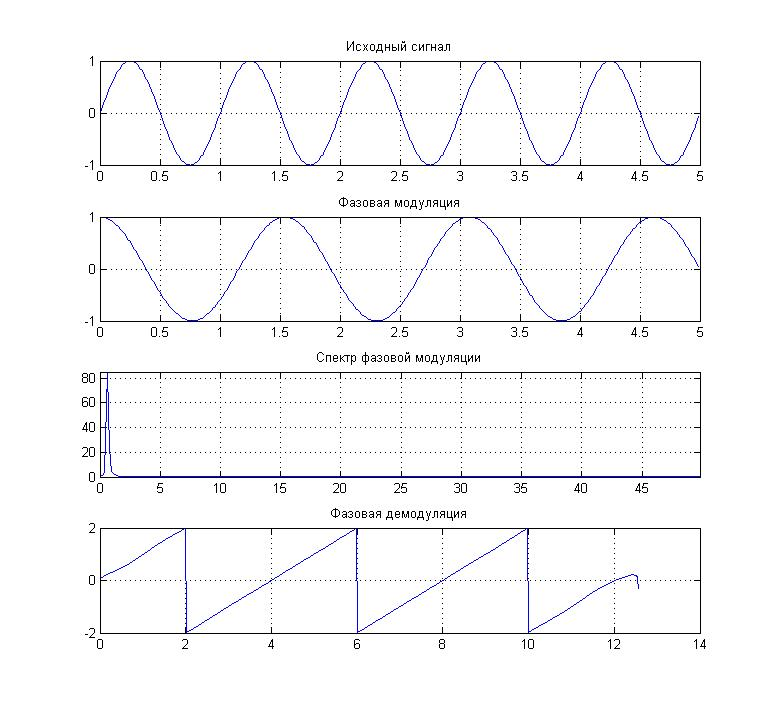
\includegraphics[width=10cm]{pm}
	\caption{Результаты фазовой модуляции/демодуляции}\label{fig.pm}
\end{figure}                                                                                                                                                                                                                                                                                                                                                                                                                                                                                                                                                                                                                                                                                                                                                                                                                                                                                                                                                                                                                                                                                                                                                                                                                                                                                                                                                                                                                                                                        
\FloatBarrier

Частотная модуляция – процесс изменения мгновенной частоты несущего колебания в соответствии с изменением информационного сигнала.По сравнению с амплитудной модуляцией здесь амплитуда остаётся постоянной.

Реализация частотной модуляции/демодуляции с помощью MATLAB:
\begin{verbatim}
% Исходный сигнал
x = 0:0.01:4*pi;
y = sin(2*pi*x);

figure
subplot(4, 1, 1);
plot(x(1:500), y(1:500))
grid
title('Исходный сигнал')
 
% Частотная модуляция
freqdev = 20;                	% Девиация частоты для частотной модуляции
fm_y = fmmod(x,Fc,Fs,freqdev); 	% Частотная модуляция
subplot(4, 1, 2);
plot(x(1:500), fm_y(1:500))
grid
title('Частотная модуляция')
spectrum = fft(fm_y, 512);      % Спектр частотной модуляции
norm_spectrum = spectrum.*conj(spectrum)/512;  
f = 100*(0:255)/512;
subplot(4, 1, 3);
plot(f, norm_spectrum(1:256))
grid
title('Спектр частотной модуляции')
axis([min(f) max(f) 0 max(norm_spectrum)]);
fdm_y = fmdemod(fm_y,Fc,Fs,freqdev); 	% Демодуляция
subplot(4, 1, 4);
plot(x, fdm_y)
grid
title('Частотная демодуляция')

\end{verbatim}


В результате выполнения приведенного кода были получены следующие характеристики:

\begin{figure}[h]\centering
	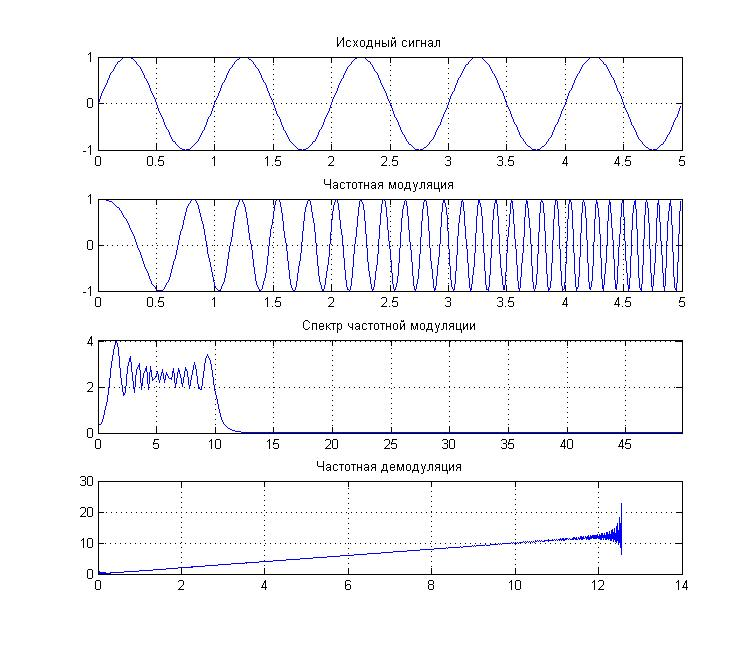
\includegraphics[width=10cm]{fm}
	\caption{Результаты частотной модуляции/демодуляции}\label{fig.fm}
\end{figure}                                                                                                                                                                                                                                                                                                                                                                                                                                                                                                                                                                                                                                                                                                                                                                                                                                                                                                                                                                                                                                                                                                                                                                                                                                                                                                                                                                                                                                                                        
\FloatBarrier

Для создания содели в Simulinc использовался раздел Communication Blockset Simulink. Выполнена модуляция, в том числе с помощью блока захваты фазы Phase-Locked Loop.

Для моделирования использоовался исходный сигнал, представленный на Рис. 51.

\begin{figure}[h]\centering
    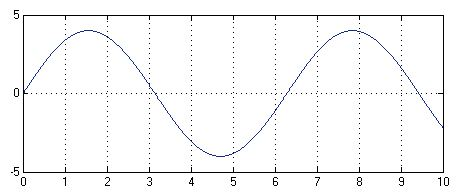
\includegraphics[width=7cm]{sim_y} 
    \caption{Исходный сигнал}\label{fig.sim_y}
\end{figure}                                                                                                                                                                                                                                                                                                                                                                                                                                                                                                                                                                                                                                                                                                                                                                                                                                                                                                                                                                                                                                                                                                                                                                                                                                                                                                                                                                                                                                                                       
\FloatBarrier

Фазовая модуляция/демодуляция в Simulink:
\begin{figure}[h]\centering
    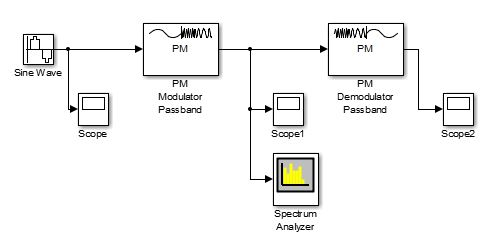
\includegraphics[width=7cm]{sim_p} 
    \caption{Фазовая модуляция/демодуляция}\label{fig.sim_p}
\end{figure}                                                                                                                                                                                                                                                                                                                                                                                                                                                                                                                                                                                                                                                                                                                                                                                                                                                                                                                                                                                                                                                                                                                                                                                                                                                                                                                                                                                                                                                                       

В результате были получены следующие характеристики:
\begin{figure}[h]\centering
  \parbox[b]{0.49\textwidth}{\centering
    \includegraphics[width=6.5cm]{sim_pm} 
    \caption{ФМ-сигнал}\label{fig.sim_pm}}
  \hfil\hfil 
  \begin{minipage}[b]{0.49\textwidth}
	\centering
	\includegraphics[width=6.5cm]{sim_pms}
	\caption{Спектр ФМ-сигнала}\label{fig.sim_pms} 
  \end{minipage}
\end{figure}

\begin{figure}[h]\centering
    \includegraphics[width=7cm]{sim_pdm} 
    \caption{Думодулированный ФМ-сигнал}\label{fig.sim_pdm}
\end{figure}
\FloatBarrier
\subsection{Выводы}

Частотная модуляция/демодуляция в Simulink:
\begin{figure}[h]\centering
    \includegraphics[width=7cm]{sim_f} 
    \caption{Частотная модуляция/демодуляция}\label{fig.sim_f}
\end{figure}                                                                                                                                                                                                                                                                                                                                                                                                                                                                                                                                                                                                                                                                                                                                                                                                                                                                                                                                                                                                                                                                                                                                                                                                                                                                                                                                                                                                                                                                       

В результате были получены следующие характеристики:
\begin{figure}[h]\centering
  \parbox[b]{0.49\textwidth}{\centering
    \includegraphics[width=6.5cm]{sim_fm} 
    \caption{ЧМ-сигнал}\label{fig.sim_fm}}
  \hfil\hfil 
  \begin{minipage}[b]{0.49\textwidth}
	\centering
	\includegraphics[width=6.5cm]{sim_fms}
	\caption{Спектр ЧМ-сигнала}\label{fig.sim_fms} 
  \end{minipage}
\end{figure}

\begin{figure}[h]\centering
    \includegraphics[width=7cm]{sim_fdm} 
    \caption{Думодулированный ЧМ-сигнал}\label{fig.sim_fdm}
\end{figure}
\FloatBarrier

Фазовая автоподстройка частоты — система автоматического регулирования, подстраивающая фазу управляемого генератора так, чтобы она была равна фазе опорного сигнала, либо отличалась на известную функцию от времени. Регулировка осуществляется благодаря наличию отрицательной обратной связи. Выходной сигнал управляемого генератора сравнивается на фазовом детекторе с опорным сигналом, результат сравнения используется для подстройки управляемого генератора.

Система ФАПЧ используется для частотной модуляции и демодуляции, умножения и преобразования частоты, частотной фильтрации, выделения опорного колебания для когерентного детектирования и в других целях.

ФАПЧ сравнивает фазы входного и опорного сигналов и выводит сигнал ошибки, соответствующий разности между этими фазами. Сигнал ошибки проходит далее через фильтр низких частот и используется в качестве управляющего для генератора, управляемого напряжением (ГУН), обеспечивающего отрицательную обратную связь. Если выходная частота отклоняется от опорной, то сигнал ошибки увеличивается, воздействуя на ГУН в сторону уменьшения ошибки. В состоянии равновесия выходной сигнал фиксируется на частоте опорного.

Также в схеме ФАПЧ включен фазовый детекто, которыйсравнивает фазы двух входных сигналов. Обычно, один из них генерируется генератором сигнала, управляемым напряжением, а второй берется из внешнего источника. ФД имеет два входа, управляющих стоящей за ним схемой подстройки частоты, задача которой сделать фазы сигналов одинаковыми.

Для ФАПЧ сигнал ошибки из ФД (значение найденной разности фаз) подается на сглаживающий фильтр (фильтр нижних частот). Сигнал с фильтра подается на управляемый напряжением генератор, частота(фаза) выходного сигнала которого зависит от напряжения на входе. Сигнал с генератора по цепи обратной связи поступает назад в детектор, замыкая контур ФАПЧ.

Частотная модуляция/демодуляция с фазовой автоподстройкой частоты в Simulink:
\begin{figure}[h]\centering
    \includegraphics[width=7cm]{sim_pll} 
    \caption{Частотная модуляция/демодуляция}\label{fig.sim_pll}
\end{figure}                                                                                                                                                                                                                                                                                                                                                                                                                                                                                                                                                                                                                                                                                                                                                                                                                                                                                                                                                                                                                                                                                                                                                                                                                                                                                                                                                                                                                                                                       

В результате были получены следующие характеристики:

\begin{figure}[h]\centering
    \includegraphics[width=7cm]{sim_fpll_filt} 
    \caption{Выход фльтра}\label{fig.sim_fpll_filt}
\end{figure}
\begin{figure}[h]\centering
  \parbox[b]{0.49\textwidth}{\centering
    \includegraphics[width=6.5cm]{sim_fpll_pd} 
    \caption{Выход фазового детектора}\label{fig.sim_fm}}
  \hfil\hfil 
  \begin{minipage}[b]{0.49\textwidth}
	\centering
	\includegraphics[width=6.5cm]{sim_fpll_vco}
	\caption{Выход ГУН}\label{fig.sim_fpll_vco} 
  \end{minipage}
\end{figure}

\FloatBarrier
\subsection{Выводы}
В результате выполнения данной работы были выполнены частотная и фазовая модуляция/демодуляция, а также чатотная демодуляция с  помощью блока захвата фазы. Можно сделать вывод, что частотная и фазовая модуляция очень тесно взаимосвязаны, поскольку обе они влияют на аргумент функции cos. Поэтому эти два вида модуляции имеют общее название — угловая модуляция.Сигнал с угловой модуляцией имеет вид колебания, начальная фаза которого зависит от времени:
	\begin{equation}
	s_(t) = A_0 cos(\omega0 t + j(t)).
	\end{equation}

Различие между фазовой и частотной модуляцией заключается лишь в том, как именно начальная фаза $j(t)$ связана с модулирующим сигналом.

Для демодуляции использовалась петля ФАПЧ, состоящая из перемножителя (используемого в качестве фазового детектора), фильтра нижних частот и генератора, управляемого напряжением (ГУН). Получаемый на выходе петли ФАПЧ сигнал пропорционален отклонению мгновенной частоты модулированного сигнала от несущей частоты, поэтому при демодуляции ФМ этот сигнал можно дополнительно проинтегрировать, чтобы получить начальную фазу сигнала.

\section{Цифровая модуляция}
\subsection{Цель работы}
Изучение методов модуляции цифровых сигналов и сравнение их свойств. 
\subsection{Алгоритм работы}
\begin{itemize}
\item Получить сигналы BPSK, PSK, OQPSK, genQAM, MSK, M-FSK модуляторов 
\item Построить их сигнальные созвездия. 
\item Провести сравнение изученных методов модуляции цифровых сигналов. 
\end{itemize}
\subsection{Теоретическая часть}
В настоящее время все большая часть информации, передаваемой по разнообразным каналам связи, существует в цифровом виде. Это означает, что передаётся последовательность целых чисел, которые могут принимать значения из некоторого фиксированного конечного 
множества. Эти числа, называемые символами (symbol), поступают от источника информации с периодом T, а частота, соответствующая этому периоду, называется символьной скоростью (symbol rate): fT = 1/T.  
Последовательность передаваемых символов является дискретным сигналом. Поскольку символы принимают значения из конечного множества, этот сигнал является и квантованным, то есть его можно назвать цифровым сигналом. В данной работе рассматриваться вопросы, связанные с преобразованием этого цифрового сигнала в аналоговый 
модулированный сигнал. 
Типичный подход при осуществлении передачи дискретной последовательности символов состоит в следующем. Каждому из возможных значений символа сопоставляется некоторый набор параметров несущего колебания. Эти параметры поддерживаются постоянными в течение 
интервала T, то есть до прихода следующего символа. Фактически это означает преобразование последовательности чисел {nk} в ступенчатый сигнал sn(t) : 
sn(t) = f(nk), kT <= t < (k + 1)T. 
Здесь f — некоторая функция преобразования. Полученный сигнал sn(t)далее используется в качестве модулирующего сигнала обычным способом. 
Такой способ модуляции, когда параметры несущего колебания меняются скачкообразно, называется манипуляцией (keying). В зависимости от того, какие именно параметры изменяются, различают амплитудную (АМн),фазовую (ФМн), частотную (ЧМн) и квадратурную (КАМн) 
манипуляцию. 
Цифровая модуляция и демодуляция включают в себя две стадии. При модуляции цифровое сообщение сначала преобразуется в аналоговый модулирующий сигнал с помощью функции modmap, а затем осуществляется аналоговая модуляция. При демодуляции сначала получается аналоговый демодулированный сигнал, а затем он преобразуется в цифровое сообщение с помощью функции demodmap.  
Функция randerr предназначена для формирования ошибок в цифровом сигнале. Она дает матрицу, в каждой строке которой имеется заданное число случайно расположенных ненулевых элементов. Для оценки помехоустойчивости системы связи необходимо произвести сравнение 
исходного (передаваемого) сообщения с сообщением, полученным в результате приема, и определить число ошибок, возникших в процессе передачи, а также вероятность ошибки. Эти действия выполняются функциями symerr и biterr, первая из которых подсчитывает число 
несовпадающих символах в двух сообщениях, а вторая — число несовпадающих битов в двоичных представлениях этих символов. Кроме числа ошибок, обе функции могут возвращать долю ошибок в общем числе символов (битов) и индикаторы мест возникновения ошибок. 
Последние две функции данной группы предназначены для графического отображения сигналов с квадратурной манипуляцией. Функция eyediagram выводит так называемую глазковую диаграмму, а функция scatterplot — диаграмму рассеяния. 
Аналоговый несущий сигнал модулируется цифровым битовым потоком.
Существуют три фундаментальных типа цифровой модуляции (или шифтинга) и один гибридный:
\begin{enumerate}
    \item ASK – Amplitude shift keying (Амплитудная двоичная модуляция).
    \item FSK – Frequency shift keying (Частотая двоичная модуляция).
    \item PSK – Phase shift keying (Фазовая двоичная модуляция).
    \item ASK/PSK.
\end{enumerate}
Одна из частных реализаций схемы ASK/PSK, которая называется QAM - Quadrature Amplitude Modulation (квадратурная амплитудная модуляция (КАМ). Это метод объединения двух AM-сигналов в одном канале. Он позваляет удвоить эффективную пропускную способность. В QAM используется две несущих с одинаковой частотой но с разницей в фазе на четверть периода (отсюда и возникает слово квадратура). 
Частотная модуляция представляет логическую единицу интервалом с большей частотой, чем ноль.
Фазовый шифтинг представляет «0» как сигнал без сдвига, а «1» как сигнал со сдвигом.

BPSK : используется единственный сдвиг фазы между «0» и «1» — 180 градусов, половина периода.
Существуют также QPSK:
QPSK использует 4 различных сдвига фазы (по четверти периода) и может кодировать 2 бита в символе (01, 11, 00, 10). 
\subsection{Код MATLAB}
\subsubsection{BPSK modulation}
h = modem.pskmod('M', 4);\newline 
g = modem.pskdemod('M', 4); \newline
msg = randint(10,1,2); \newline
modSignal = modulate(h,msg); \newline
errSignal = (randerr(1,10, 3) ./ 30)';\newline 
modSignal = modSignal + errSignal; \newline
demodSignal = demodulate(g,modSignal); \newline
scatterplot(modSignal);\newline
\begin{figure}[h]
\centering
\includegraphics[width=10cm]{1_1.png} 
\caption{Временная характеристика чистого синусоидального сигнала} 
\end{figure}
\newpage
\FloatBarrier
\subsubsection{PSK modulation}
h = modem.pskmod('M', 8); \newline
g = modem.pskdemod('M', 8); \newline
msg = randint(10,1,8); \newline
modSignal = modulate(h,msg); \newline
errSignal = (randerr(1,10, 3) ./ 30)'; \newline
modSignal = modSignal + errSignal; \newline
demodSignal = demodulate(g,modSignal); \newline
scatterplot(modSignal);\newline
\begin{figure}[h]
\centering
\includegraphics[width=10cm]{1_2.png} 
\caption{Временная характеристика чистого синусоидального сигнала} 
\end{figure}
\newpage
\FloatBarrier
\subsubsection{OQPSK modulation}
h = modem.oqpskmod; \newline
g = modem.oqpskdemod; \newline
msg = randint(200,1,4); \newline
modSignal = modulate(h,msg); \newline
errSignal = (randerr(1,400, 100) ./ 30)';\newline 
modSignal = modSignal + errSignal; 4 \newline
demodSignal = demodulate(g,modSignal); \newline
scatterplot(modSignal);\newline
\begin{figure}[h]
\centering
\includegraphics[width=10cm]{1_3.png} 
\caption{Временная характеристика чистого синусоидального сигнала} 
\end{figure}
\newpage
\FloatBarrier
\subsubsection{GENQAM modulation}
M = 8; \newline
h = modem.genqammod('Constellation', exp(j*2*pi*[0:M-1]/M)); \newline
g = modem.genqamdemod('Constellation', exp(j*2*pi*[0:M-1]/M)); \newline
msg = randint(8,1,8);\newline 
modSignal = modulate(h,msg); \newline
errSignal = (randerr(1,8, 3) ./ 30)';\newline 
modSignal = modSignal + errSignal; \newline
demodSignal = demodulate(g,modSignal); \newline
scatterplot(modSignal);\newline
\begin{figure}[h]
\centering
\includegraphics[width=10cm]{1_4.png} 
\caption{Временная характеристика чистого синусоидального сигнала} 
\end{figure}
\newpage
\FloatBarrier
\subsubsection{MSK modulation}
h = modem.mskmod('SamplesPerSymbol', 3); \newline
g = modem.mskdemod('SamplesPerSymbol', 3); \newline
msg = randint(3,1,2); \newline
modSignal = modulate(h, msg); \newline
errSignal = (randerr(1,9, 3) ./ 30)'; \newline
modSignal = modSignal + errSignal; \newline
demodSignal = demodulate(g, modSignal); \newline
scatterplot(modSignal); \newline
\begin{figure}[h]
\centering
\includegraphics[width=10cm]{1_5.png} 
\caption{Временная характеристика чистого синусоидального сигнала} 
\end{figure}
\subsection{Работа в среде Simulink}
\subsubsection{BPSK modulation}
\begin{itemize}
\item Получен сигнал BPSK и построено сигнальное созвездие в среде Simulink
\begin{figure}[h]
\centering
\includegraphics[width=11cm]{sim1_1.png} 
\end{figure}
\item Сигнальное созвездие
\begin{figure}[h]
\centering
\includegraphics[width=9cm]{sim1.png} 
\end{figure}
\end{itemize}
\newpage
\FloatBarrier
\subsubsection{DBPSK modulation}
\begin{itemize}
\item Получен сигнал DBPSK и построено сигнальное созвездие в среде Simulink
\begin{figure}[h]
\centering
\includegraphics[width=12cm]{sim2_1.png} 
\end{figure}
\item Сигнальное созвездие
\begin{figure}[h]
\centering
\includegraphics[width=12cm]{sim2.png} 
\end{figure}
\end{itemize}
\newpage
\FloatBarrier
\subsubsection{M-FSK modulation}
\begin{itemize}
\item Получен сигнал M-FSK и построено сигнальное созвездие в среде Simulink
\begin{figure}[h]
\centering
\includegraphics[width=12cm]{sim3_1.png} 
\end{figure}
\item Сигнальное созвездие
\begin{figure}[h]
\centering
\includegraphics[width=12cm]{sim3.png} 
\end{figure}
\end{itemize}
\subsection{Вывод}
Уровень модуляции определяет количество состояний несущей, используемых для передачи информации. Чем выше этот уровень, тем большими скоростными возможностями и меньшей помехоустойчивостью модуляция обладает. Число бит, передаваемых одним состоянием, 
определяется как Log N, где N — уровень модуляции. Таким образом, чем выше уровень модуляции, тем больше данных мы можем передать (или потерять) за единицу времени. 

\end{document}